\documentclass[10pt,oneside,a4paper]{article}
\usepackage[left=2cm,right=2cm,top=2cm,bottom=1cm,includeheadfoot]{geometry}
\usepackage{ngerman}
\usepackage[utf8]{inputenc}
% \usepackage{amsfonts,amssymb,amsmath,cancel,graphicx,textcomp}
\usepackage{amsfonts,amssymb,amsmath,graphicx,textcomp}
\usepackage{float}
\usepackage{color,xcolor}
\usepackage{url}
\usepackage{hyperref}
\usepackage{listings}
\usepackage{tikz}
\usepackage{fancyhdr}
\usepackage{gensymb}
\usepackage[section]{placeins}
\usetikzlibrary{arrows,shapes,snakes,automata,backgrounds,petri,positioning}

\hypersetup{
    colorlinks,
    citecolor=black,
    filecolor=black,
    linkcolor=black,
    urlcolor=black
}

\pagestyle{fancy}
\fancyhf{}
\fancyhead[L]{crash override : \\Steve Dierker, Semjon Kerner, Artur Jeske}
\fancyhead[C]{"Ubungsblatt 07}
\fancyhead[R]{Seite \thepage}
\renewcommand{\headrulewidth}{0.5pt}

% lstlisting mit Zeilennummerierung und grauen Kommentaren, Zeilenumbruch, etc. pp.
\lstset{
  numbers=left, numberstyle=\tiny, numbersep=5pt,
  tabsize=2,
  breaklines=true, breakindent=0pt, postbreak=\mbox{$\rightarrow\ \ $},
  showstringspaces=false,
  extendedchars=false,
  basicstyle=\small\ttfamily,
  commentstyle=\color{black!40},
  stringstyle=\color{black!40!blue},
  keywordstyle=\color{black!40!green}
}

% Komma Abstände bei Tausendern/Dezimalzahlen ans dt. anpassen
\mathcode`,="013B
\setlength{\parindent}{0em}
\setlength{\parskip}{0.5em}

\begin{document}
  \section{Map description}
    \begin{figure}[h]
      \centering
      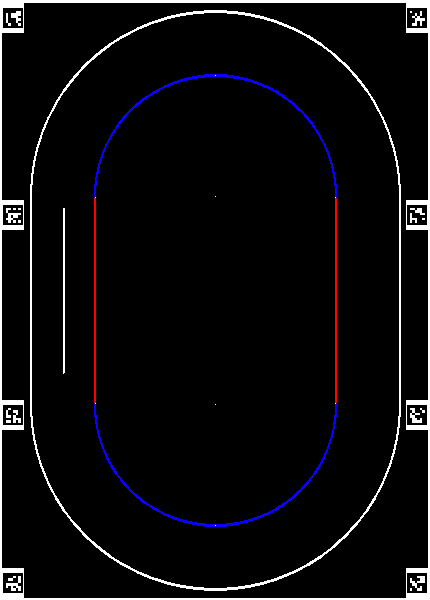
\includegraphics[scale=0.5]{pictures/map.png}
      \caption{Karte mit eingezeichneten Me"spunkten.}
    \end{figure}
    \begin{itemize}
      \item{Linie links:} \( P_{1L} = (95.5, 197); P_{2L} = (95.5, 403) \) \\
        \( x = 95,5 \)
      \item{Linie rechts:} \( P_{1R} = (335.5, 197); P_{2R} = (335.5, 403) \) \\
        \( x = 335,5 \)
      \item{Kreis oben:} \( P_{CO} = (215, 196), r = 120 \) \\
        \( (x - 215)^2 + (y - 196)^2 = 120^2 \)
      \item{Kreis unten:} \( P_{CU} = (215, 404), r = 120 \) \\
        \( (x - 215)^2 + (y - 404)^2 = 120^2 \)
    \end{itemize}

  \section{Closest point on trajectory}

  \section{Ceilin camera GPS}
\end{document}
